\documentclass{beamer}
\usepackage{graphicx}
\usepackage{amsmath}


\usetheme{m}
\title{Predicting TCP/IP Network Traffic using Time Series Forecasting}
\subtitle{Final Presentation}
\date{June 16, 2016}
\author{Thomas Mauerhofer, and Matthias Wölbitsch}


\begin{document}
  \maketitle
  
  \begin{frame}{Recap}   
    \textbf{goal: forecast TCP/IP traffic}
    \begin{itemize}
     \item real-time and short-time
    \end{itemize}
    
    \textbf{data set}
    \begin{itemize}
     \item network traffic of three months
    \end{itemize}
    
    \textbf{approaches}
    \begin{itemize}
     \item classical time series prediction methods
     \item artificial neural networks
    \end{itemize}
  \end{frame}
 
 
  \begin{frame}{Neural Network Approach}
    \textbf{data set preparation}
    \begin{itemize}
     \item generate sequences using sliding window 
     \item split into training, validation, and test set
    \end{itemize}
  
    \textbf{neural network library}
    \begin{itemize}
      \item keras 
      \item theano
    \end{itemize}
    
    \textbf{hyper parameter search}
    \begin{itemize}
     \item sliding window, number of neurons, number of layers,\ldots
     \item hyperopt library
     \item tree-structured parzen estimator
    \end{itemize}
  \end{frame}
  
  
  \begin{frame}{Results}
    \begin{columns}[c]
      \column{0.35\textwidth}  
      \textbf{MLP}
      \begin{itemize}
	\item \(N=25\)
	\item \(W = \{1,2,4,8\} \cup \{287,288,289\}\)
      \end{itemize}
    
      \textbf{1 layer LSTM}
      \begin{itemize}
	\item \(N = 19\)
	\item \(W = \{1,2,\ldots,19\}\)
      \end{itemize}
      
      \textbf{2 layer LSTM}
      \begin{itemize}
	\item \(N_1 = 13\)
	\item \(N_2 = 5\)
	\item \(W = \{1,2,\ldots,14\}\)
      \end{itemize}
    
      \column{0.65\textwidth} 
      \textbf{forecast error for different horizons}
      \begin{figure}
	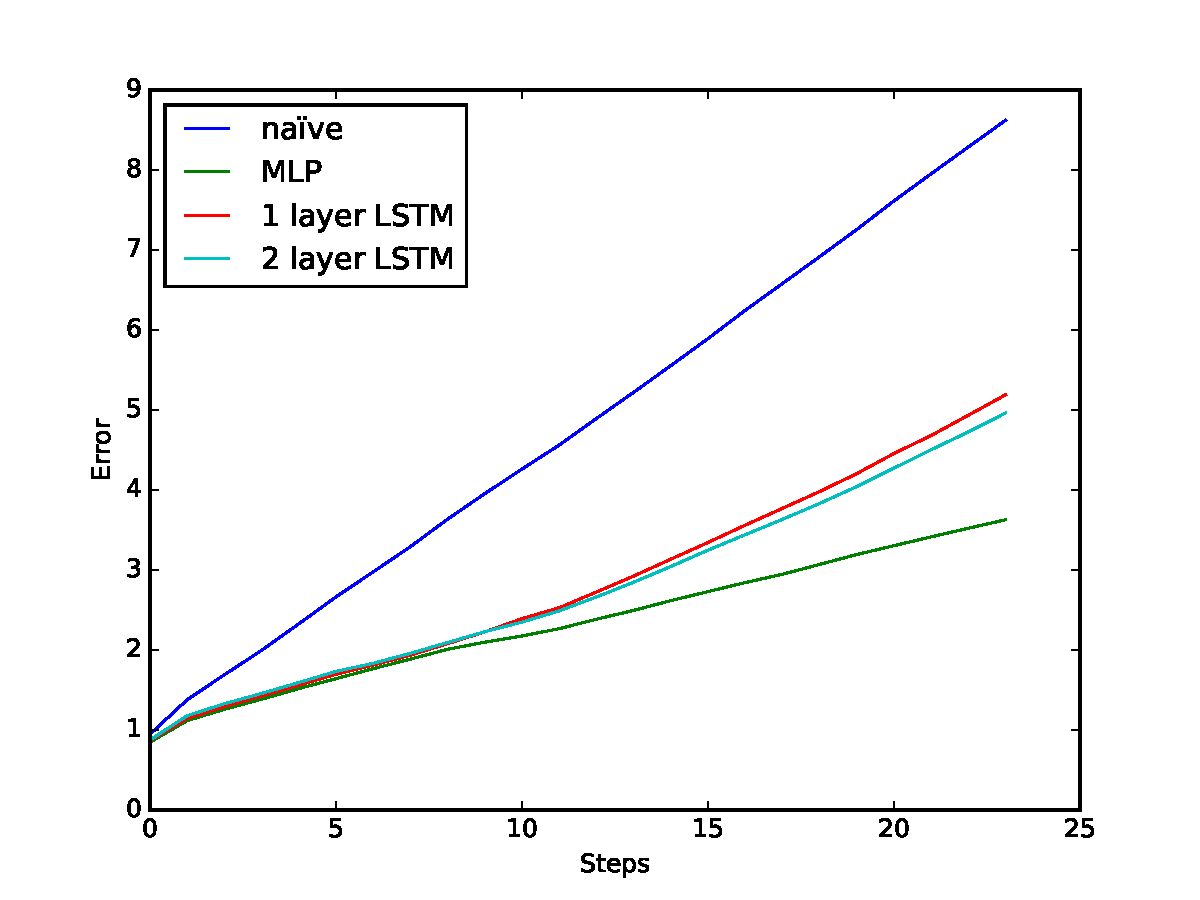
\includegraphics[width=1.1\textwidth]{images/nn_errors.pdf}
      \end{figure}
    \end{columns}
  \end{frame}
  
  \begin{frame}{Results}
    \textbf{forecasting examples with \(h=1\) and \(h=24\) using MLP}
    
    \begin{columns}[c]
      \column{0.5\textwidth}  
      \begin{figure}
       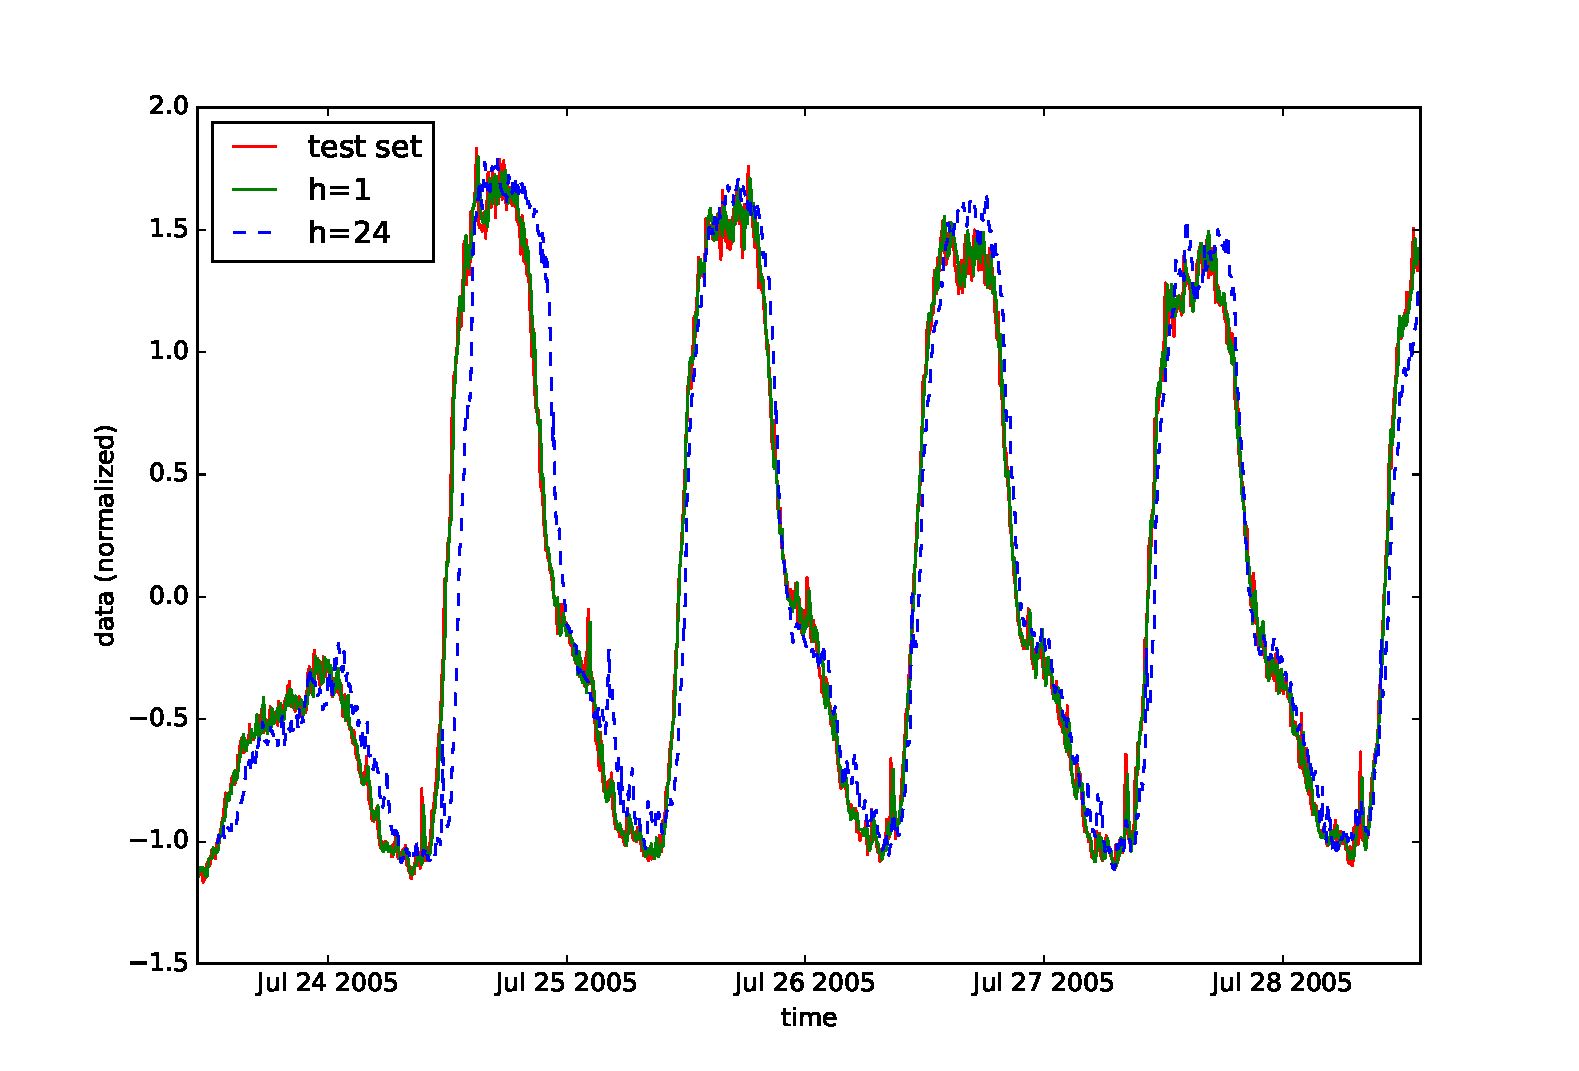
\includegraphics[width=1.1\textwidth]{images/example_forecast.pdf}
      \end{figure}

      \column{0.5\textwidth}
       \begin{figure}
        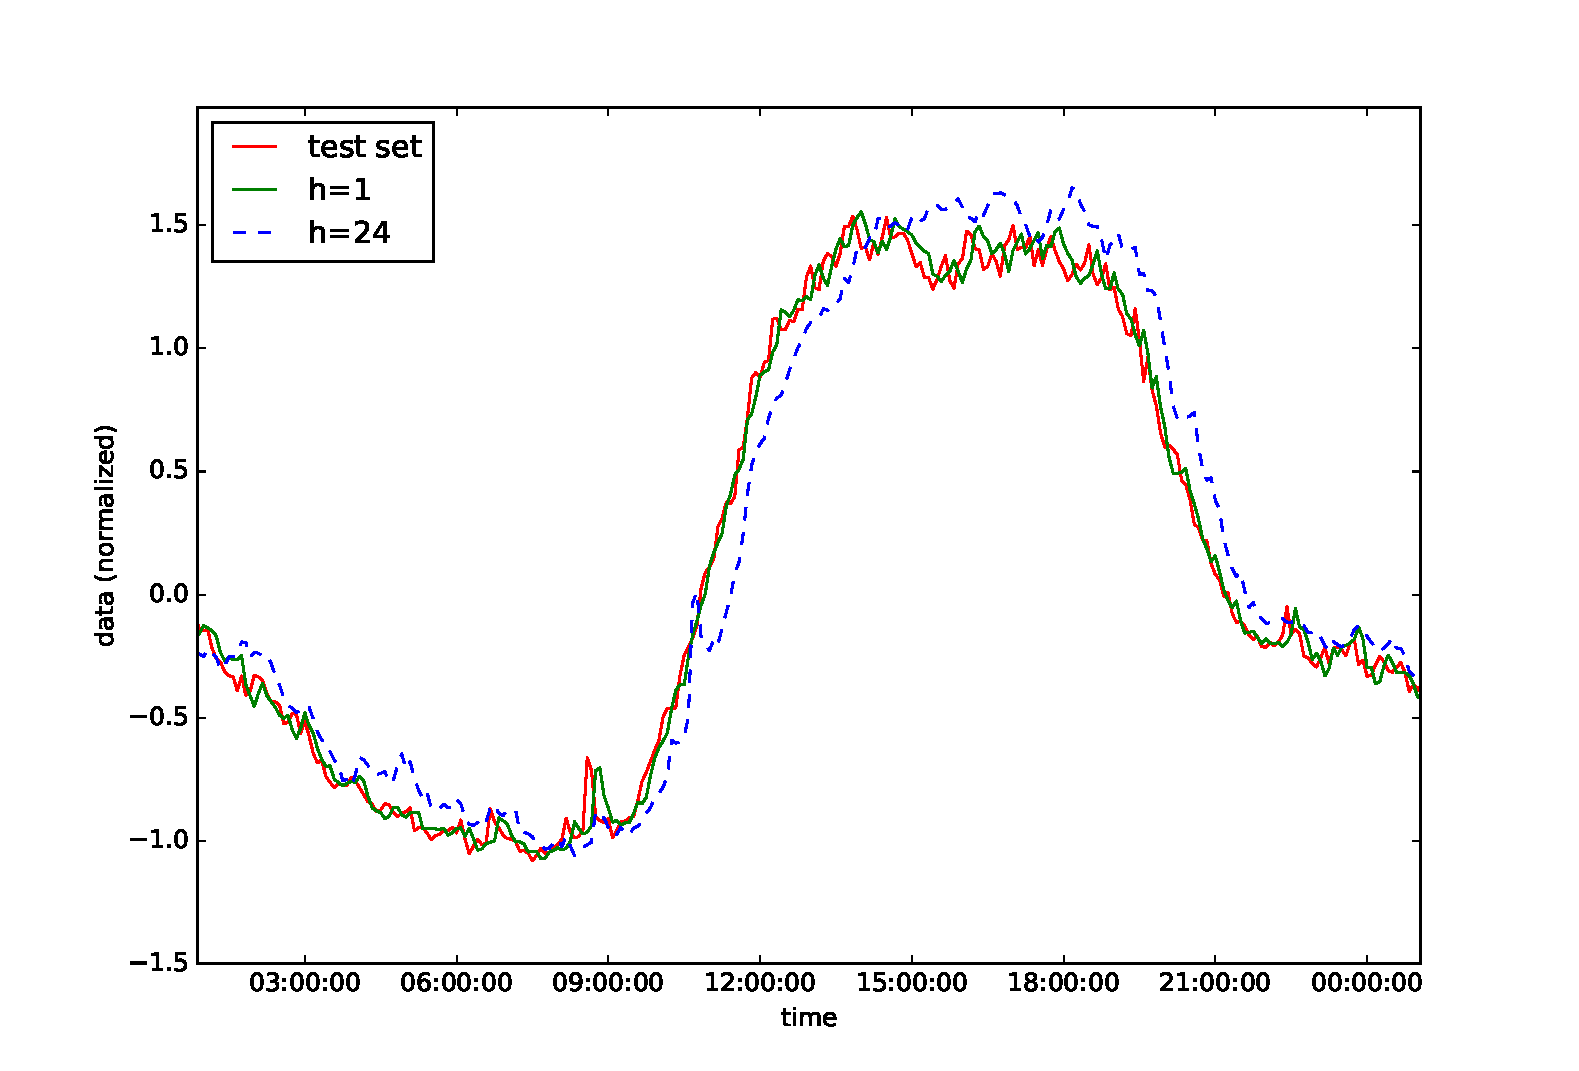
\includegraphics[width=1.1\textwidth]{images/example_forecast_day.pdf}
       \end{figure}
    \end{columns}
  \end{frame}
  
  
  \begin{frame}{Conclusion}  
    \begin{columns}[c]
      \column{0.5\textwidth}  
      \textbf{forecast horizon}
      \begin{itemize}
       \item one step ahead forecasting
       \item direct vs. iterative forecasting
      \end{itemize}
      
      \hspace{10pt}
      
      \textbf{training loss function}
      \begin{itemize}
       \item MSLE 
       \item penalizes underestimates
       \item numerical issues
      \end{itemize}

      \column{0.5\textwidth}
        \begin{figure}
         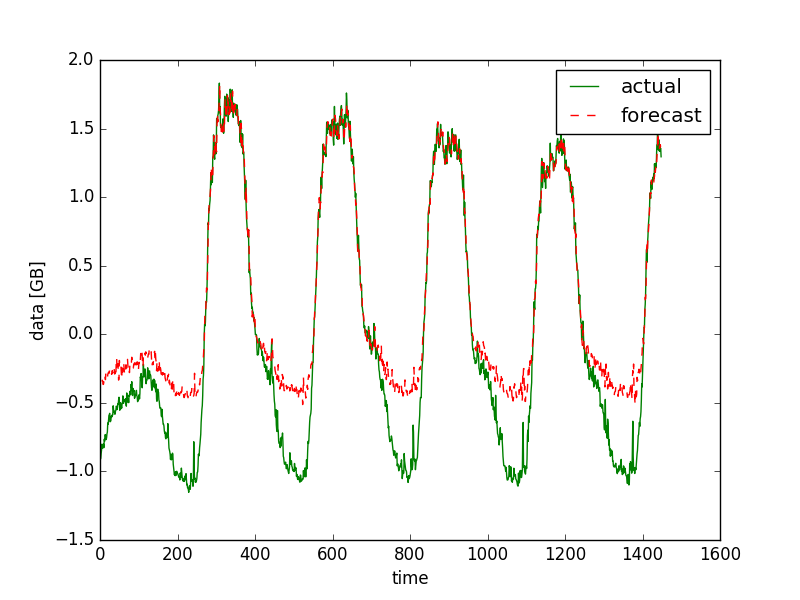
\includegraphics[width=1.0\textwidth]{images/msle_standardized_data_issue.png}
        \end{figure}
    \end{columns}
  \end{frame}
  
  
  \begin{frame}{Conclusion}
    \textbf{LSTM issues}
    \begin{itemize}
     \item high expectations
     \item too few training samples
     \item slow
    \end{itemize}
    
    \textbf{neural networks and time series}
    \begin{itemize}
     \item used often for forecasting
     \item numerous different approaches
     \item problem solved?
    \end{itemize}

  \end{frame}


  \plain{Questions?}
\end{document}